% Created 2024-08-03 Sat 04:45
% Intended LaTeX compiler: pdflatex
\documentclass[aspectratio=169,xcolor={dvipsnames,svgnames}]{beamer}
\usepackage[utf8x]{inputenc}
\usepackage[T1]{fontenc}
\usepackage{graphicx}
\usepackage{longtable}
\usepackage{wrapfig}
\usepackage{rotating}
\usepackage[normalem]{ulem}
\usepackage{amsmath}
\usepackage{amssymb}
\usepackage{capt-of}
\usepackage{hyperref}
\usepackage{minted}
\usepackage{libertine}
\usepackage[normalem]{ulem}
\usepackage{varwidth}
\usepackage[Export]{adjustbox}
%\usepackage{enumitem}
\graphicspath{ {./careful-Isaac-Images/} {./org-download-images/} }
\usepackage[date=year,%
backend=biber,%
style=alphabetic,%
maxnames=5,%
minnames=3,%
maxalphanames=4,%
minalphanames=3,%
backref=true,%
doi=false,%
isbn=false,%
url=false,%
eprint=false]{biblatex}
\DefineBibliographyStrings{english}{%
backrefpage  = {\lowercase{s}ee p.}, % for single page number
backrefpages = {\lowercase{s}ee pp.} % for multiple page numbers
}
\addbibresource{/home/bvraghav/bibliography.bib}
%% Math typesetting
%% --------------------------------
\usepackage{amsmath}
\usepackage{amssymb}
\usepackage{amsfonts}
\usepackage{bbold}
% Operators with limit-style sub and superscript
\DeclareMathOperator*{\E}{\mathbb{E}}
\hypersetup{%
colorlinks=true,%
allcolors=magenta,%
%linkbordercolor = {white},%
%<your other options...>,
}
\usetheme{boxes}
\usecolortheme{crane}
\usefonttheme{serif}
\useinnertheme{rectangles}
\useoutertheme{}
\date{}
\title{mca101 : computer graphics}
\author{%
%\noindent{} \\[2em]
\normalsize Raghav B. Venkataramaiyer
}
\institute{%
CSED TIET Patiala India.
}
\date{\scriptsize \today}
\setbeamercolor{alerted text}{fg=red!80!black}
%% Setup outline at begin section
%% -------------------------------------------------------
\AtBeginSection[]               % Section
{
\begin{frame}{outline}
\tableofcontents[currentsection,hideallsubsections]
\end{frame}
}
\AtBeginSubsection[]            % SubSection
{
\begin{frame}{outline}
\tableofcontents[currentsection,currentsubsection,subsectionstyle=show/shaded/hide]
\end{frame}
}
\setbeamerfont{structure}{shape=\scshape,family=\sffamily}
\setbeamertemplate{section page}
{
\begin{centering}
\begin{beamercolorbox}[sep=12pt,center]{part title}
\usebeamerfont{section title}\insertsection\par
\end{beamercolorbox}
\end{centering}
}

\setbeamercovered{transparent}
\hypersetup{
 pdfauthor={B.V. Raghav},
 pdftitle={mca101 : computer graphics},
 pdfkeywords={},
 pdfsubject={},
 pdfcreator={Emacs 29.4 (Org mode 9.6.24)}, 
 pdflang={English}}
\begin{document}

\maketitle

\section{history}
\label{sec:org3e6d7fa}

\subsection{Applications}
\label{sec:orgf46d8c9}

\begin{frame}[label={sec:org3bbaf97}]{sketchpad 1960}
\centering

\begin{center}
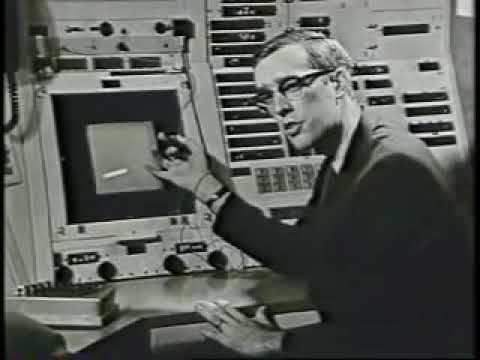
\includegraphics[width=0.5\linewidth]{images/sutherland-sketchpad.jpg}
\end{center}
\tiny \emph{Image Courtesy: \href{https://www.youtube.com/watch?v=ztRtFEwyXnY}{Youtube}}
\end{frame}

\begin{frame}[label={sec:org6d0a567}]{Flatland 1999}
\begin{figure}[htbp]
\centering
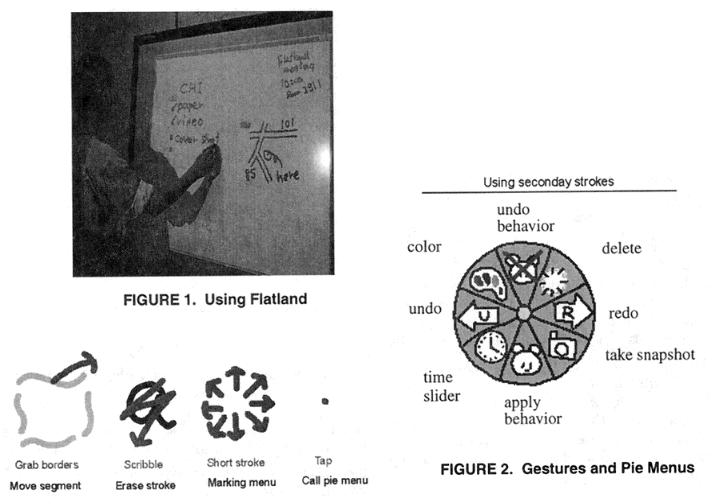
\includegraphics[width=0.6\linewidth]{images/flatland-1999.png}
\caption{Flatland \cite{MIEL99}}
\end{figure}
\end{frame}

\begin{frame}[label={sec:org05e148a}]{plushie 2007}
\centering

\begin{figure}[htbp]
\centering
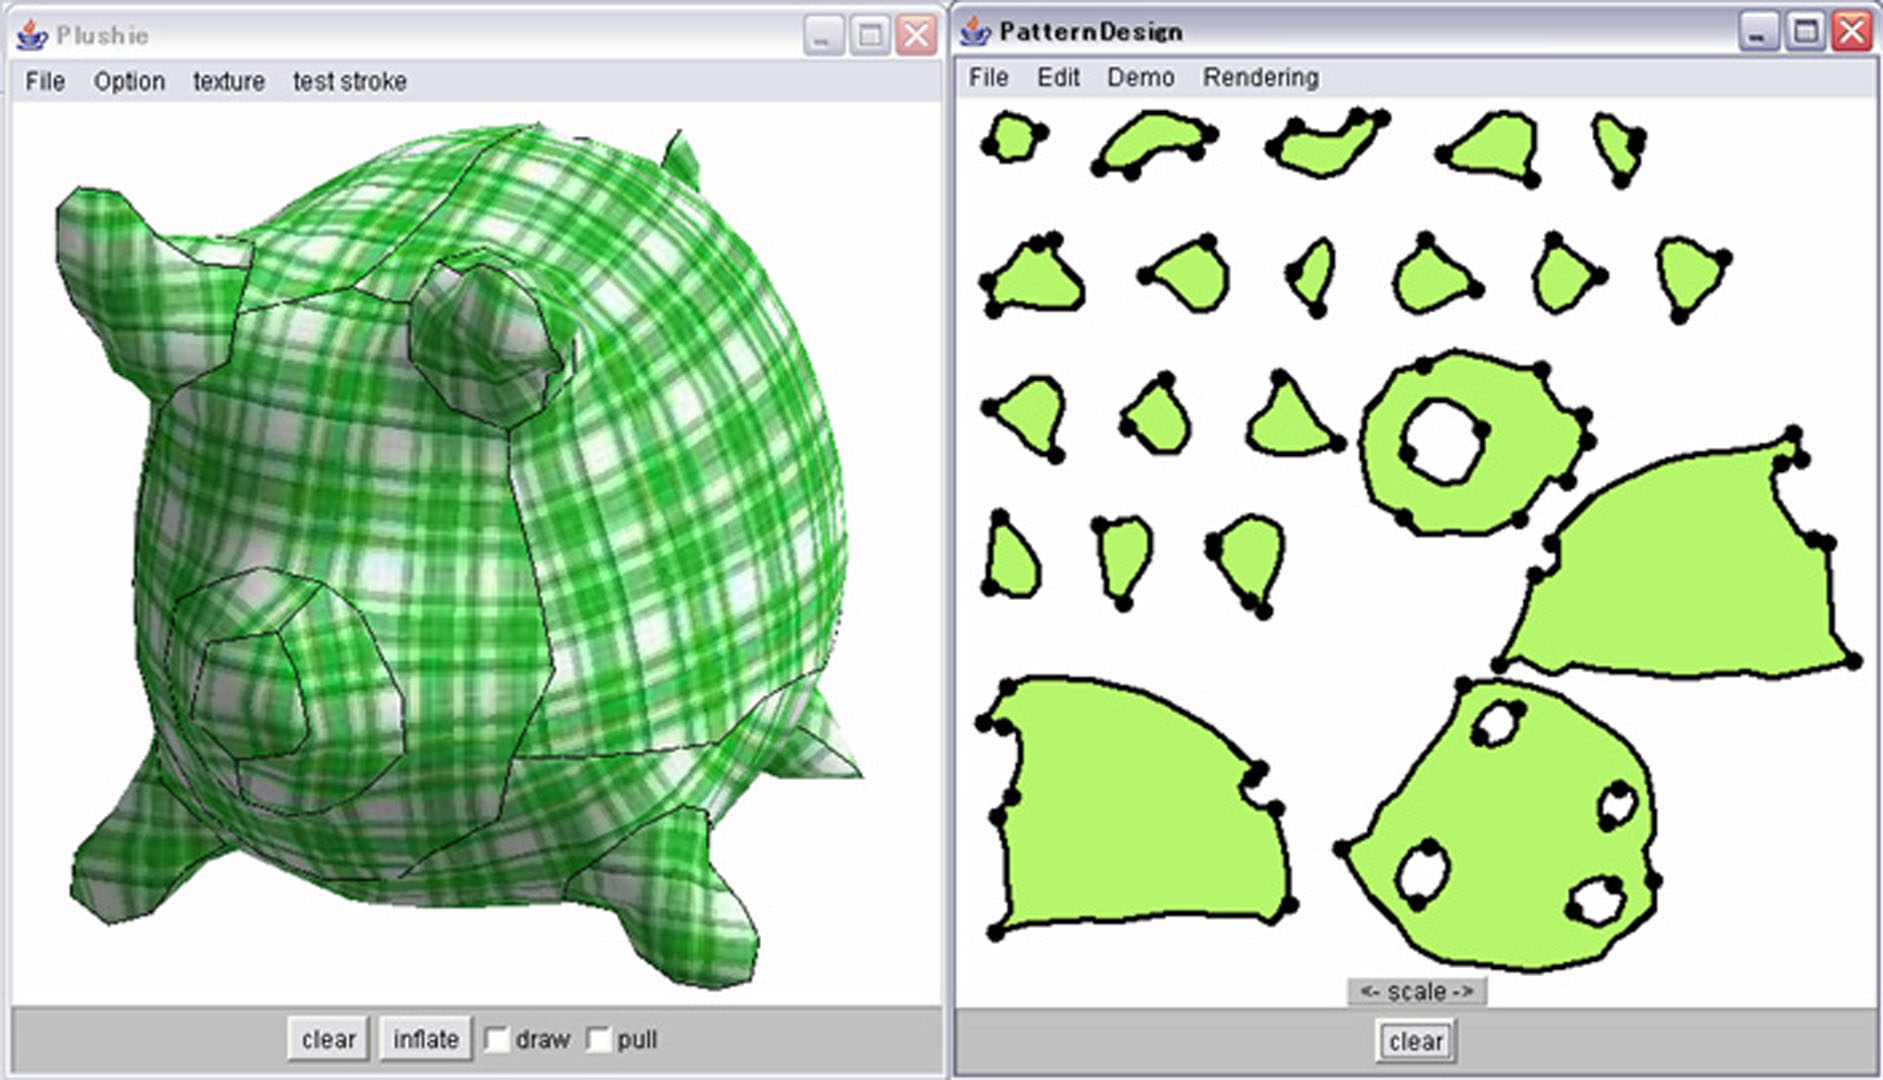
\includegraphics[width=0.6\linewidth]{images/plushie-2007.jpg}
\caption{Plushie \cite{MI07}}
\end{figure}

See Also: \href{https://www.youtube.com/watch?v=rbQWxL-\_8LU}{Teaser @Youtube}
\end{frame}

\begin{frame}[label={sec:orgde46839}]{cityengine esri 2012}
\centering

\begin{center}
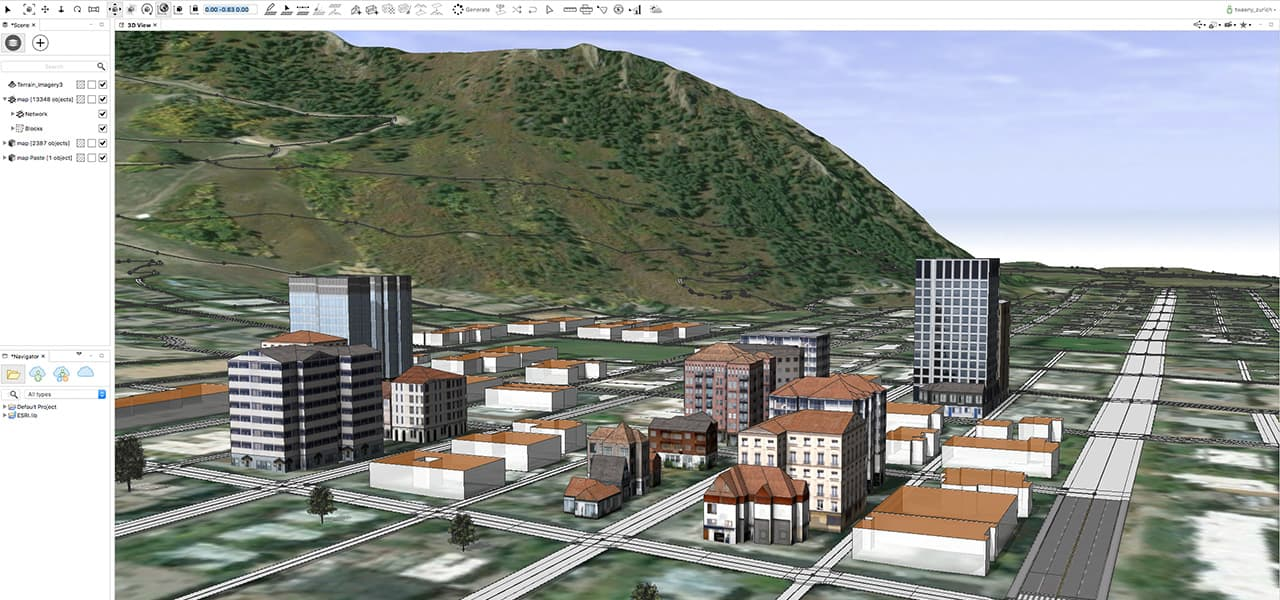
\includegraphics[width=0.8\linewidth]{images/cityengine-esri.jpg}
\end{center}
\tiny \emph{Image Courtesy: \href{https://www.youtube.com/watch?v=aFRqSJFp-I0}{Youtube}}

See Also: \href{https://www.youtube.com/watch?v=jsFztFXiPTM}{Peter Wonka @3DGV}
\end{frame}

\subsection{Display}
\label{sec:orgce45c6e}

\begin{frame}[label={sec:org1f1cbd4}]{cathode ray tube}
\centering

\begin{center}
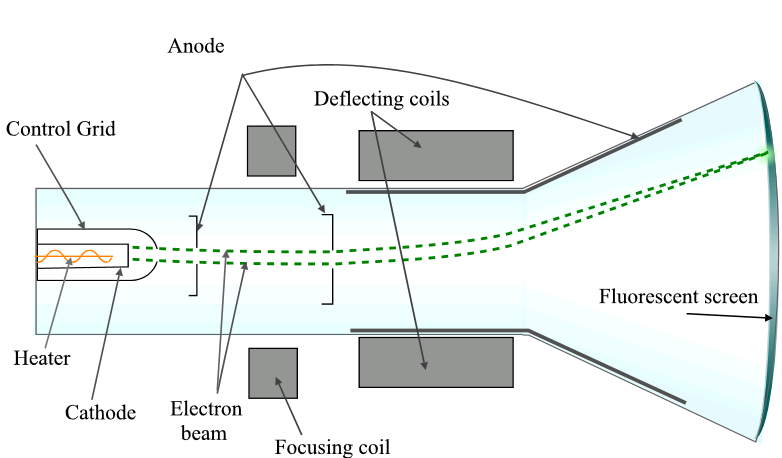
\includegraphics[width=0.6\linewidth]{images/crt.png}
\end{center}
\tiny \emph{Image Courtesy: \href{https://en.wikipedia.org/wiki/File:Cathode\_ray\_Tube.PNG}{Wikipedia}}

Monochrome (Raster), Colour (Raster), Direct-View
Bistable Storage (Vector)
\end{frame}

\begin{frame}[label={sec:org65f9fb0}]{nixie Tube}
(Variant of a Neon Lamp)
\centering

\begin{center}
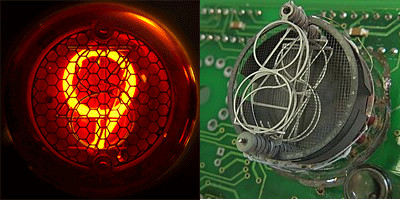
\includegraphics[width=0.6\linewidth]{images/Nixie2.jpg}
\end{center}
\tiny \emph{Image Courtesy: \href{https://en.wikipedia.org/wiki/Nixie\_tube}{Wikipedia}}
\end{frame}

\begin{frame}[label={sec:org54c236d}]{flip-disc display}
\centering

\begin{center}
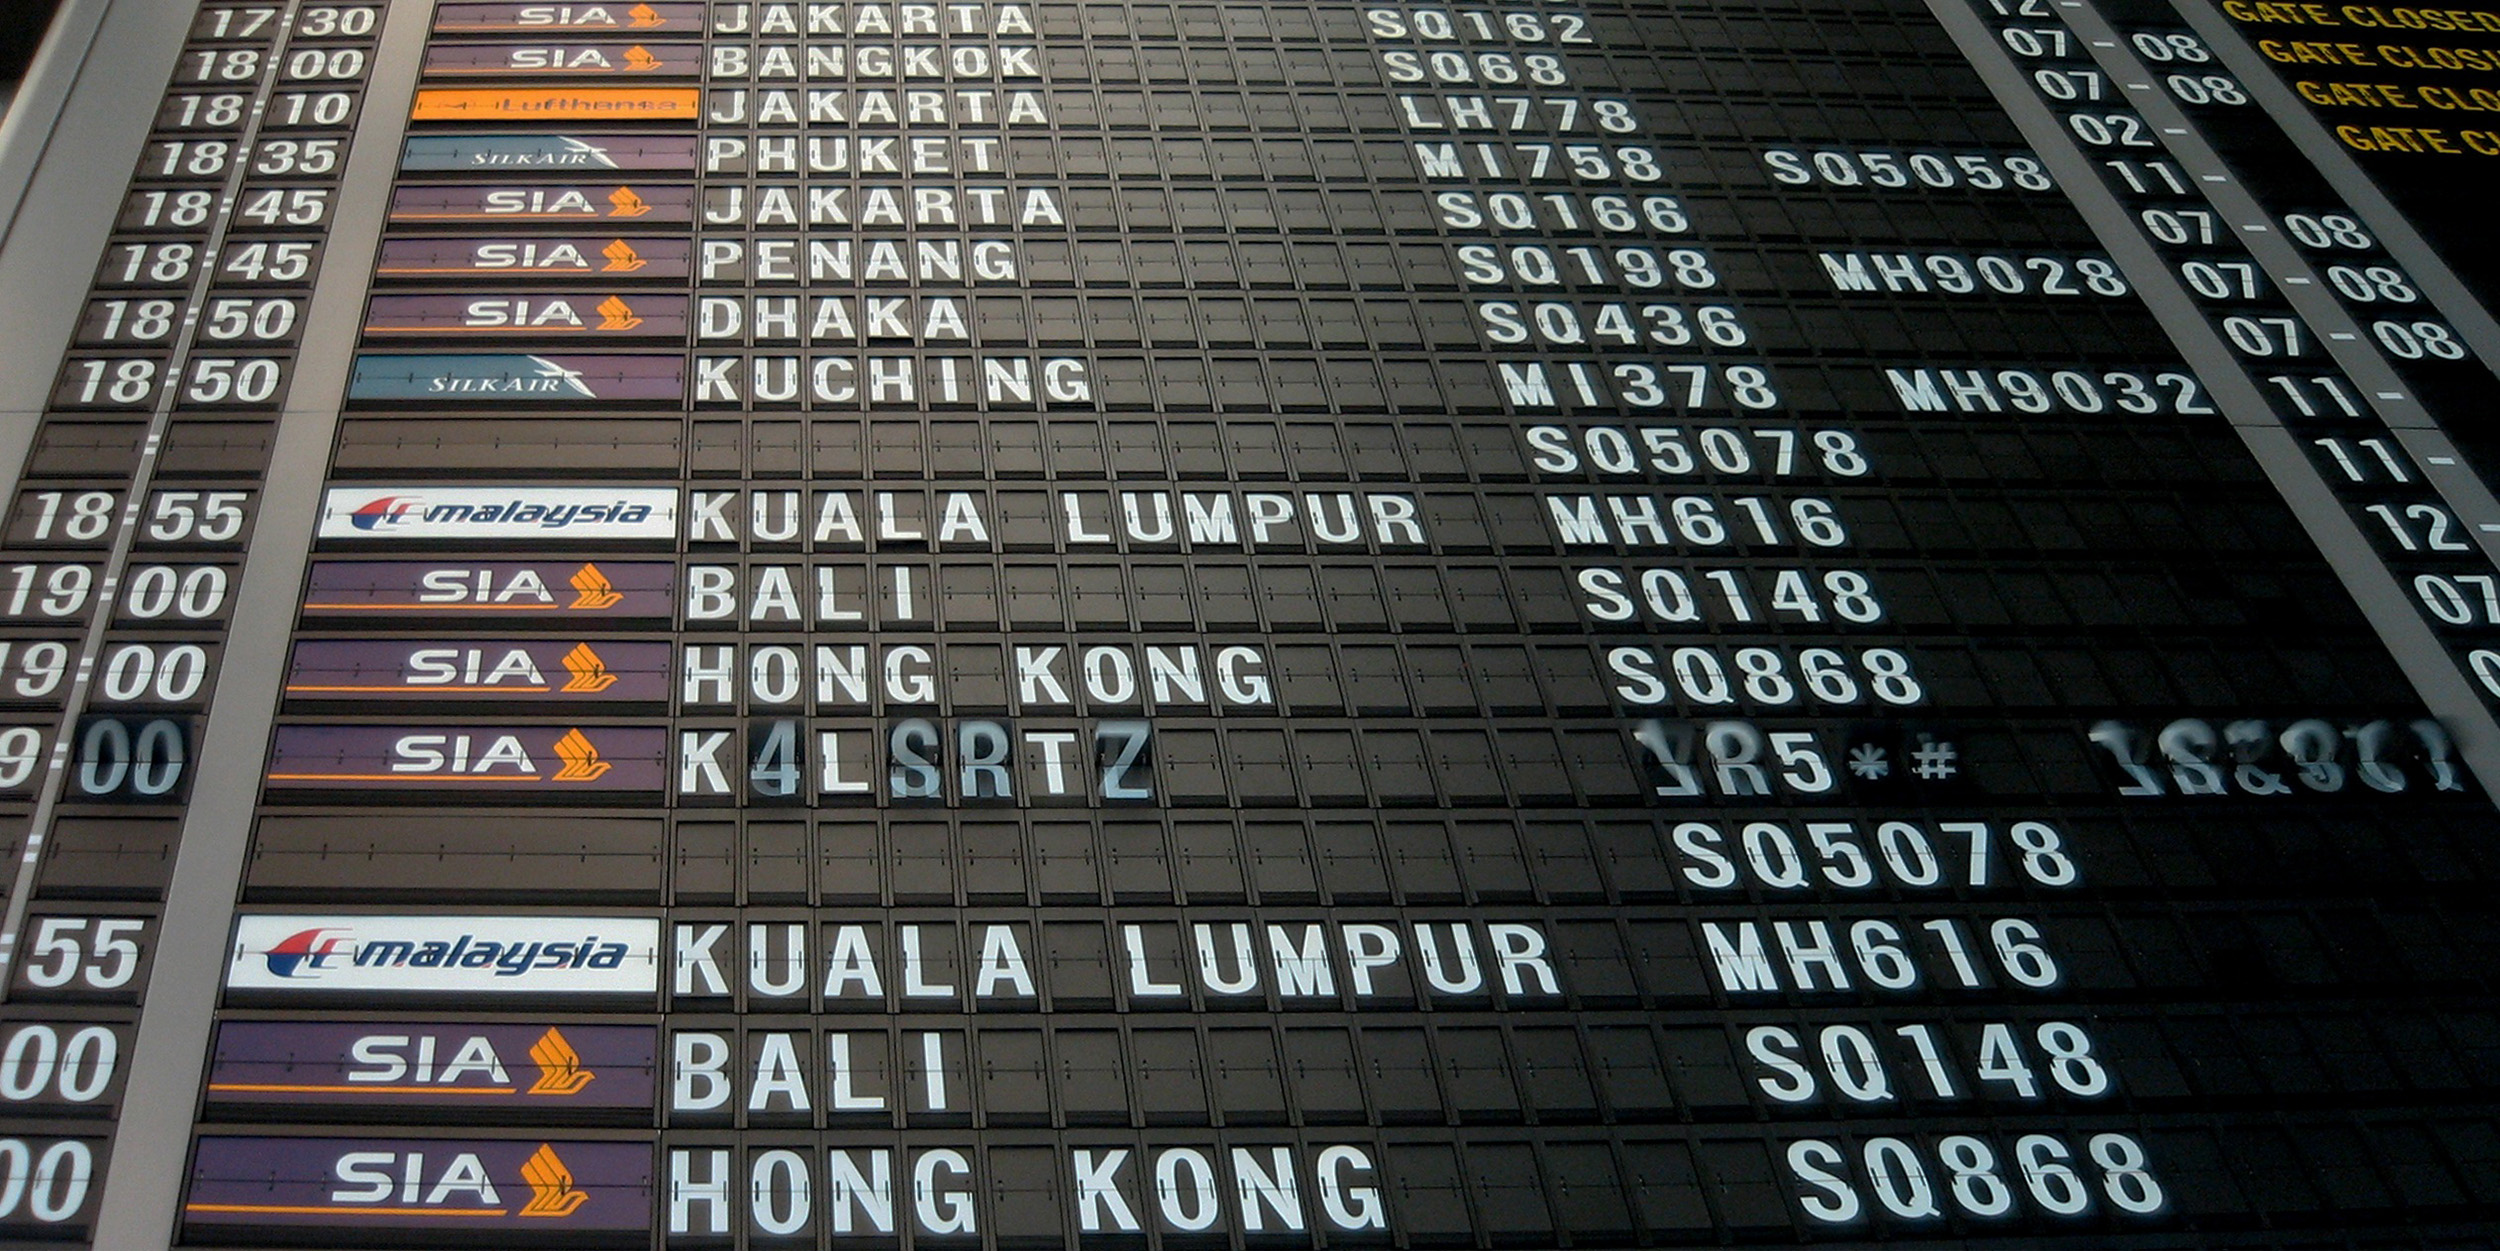
\includegraphics[width=0.8\linewidth]{images/Changi-T2-Flipboard-2.jpg}
\end{center}
\tiny \emph{Image Courtesy: \href{https://mainlymiles.com/2020/01/17/changis-iconic-flip-board-displays-to-go-as-terminal-2-revamp-gets-underway/}{Web}}
\end{frame}

\begin{frame}[label={sec:orgc05f6cb}]{Recently}
\begin{itemize}
\item LCD
\item Plasma (1995)
\item LED
\item OLED
\item AMOLED
\item E-Ink (Kindle)
\end{itemize}
\end{frame}

\subsection{Print}
\label{sec:org30b80ea}

\begin{frame}[label={sec:org73c29c6}]{raster}
\begin{columns}
\begin{column}{0.5\columnwidth}
Prehistoric, Ancient \& Medieval
\begin{itemize}
\item Clay Tablets
\item Wood Block Printing
\item Stencils/ Masks
\item Seals and Stamps
\item Lithography
\item Flat-bed Printing Press
\end{itemize}
\end{column}
\begin{column}{.5\columnwidth}
Modern
\begin{itemize}
\item Rotary Printing Press
\item Offset Press
\item Screenprinting
\item Dot matrix printing (DMP)
\item Thermal Printing (Thermochromic)
\item Laser Printing
\end{itemize}
\end{column}
\end{columns}
\end{frame}

\begin{frame}[label={sec:org6d0f03b}]{vector}
\centering

\begin{center}
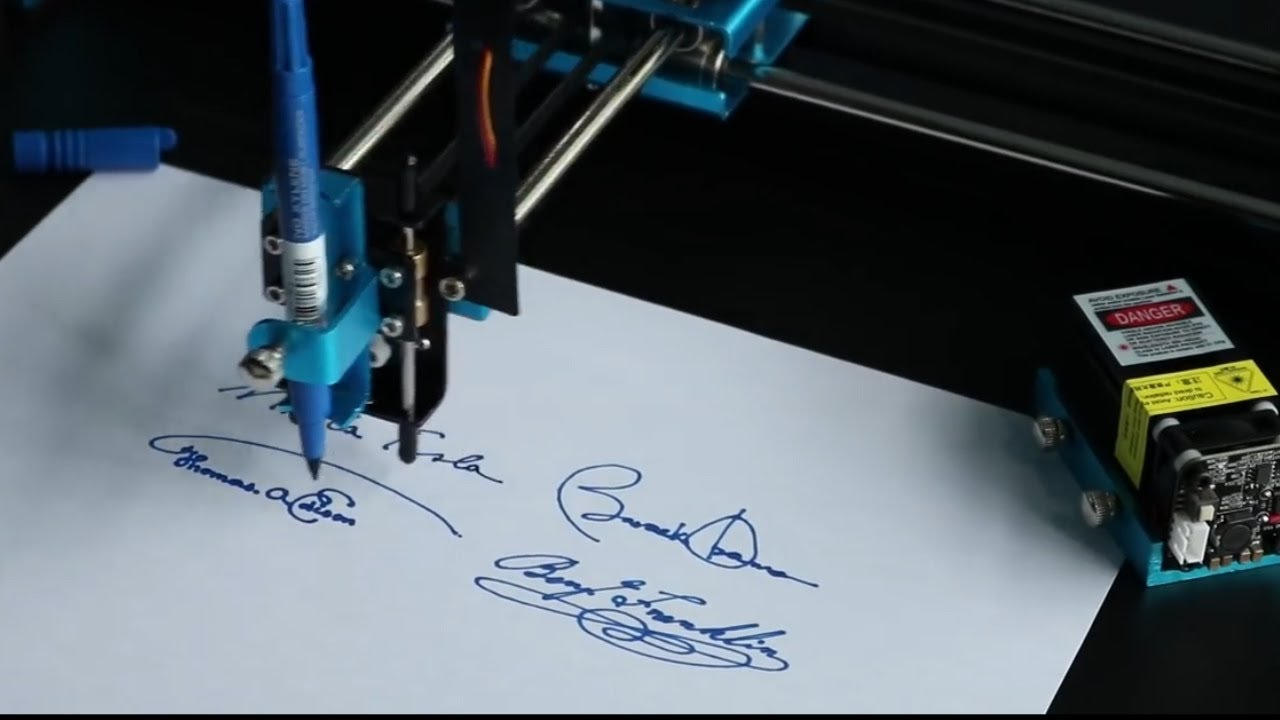
\includegraphics[width=0.6\linewidth]{images/plotter.jpg}
\end{center}
\tiny \emph{Image Courtesy: \href{https://i.ytimg.com/vi/3ohDaX4uxKY/maxresdefault.jpg}{Youtube}}

See Also: \href{https://youtu.be/nMt5Dw04XhY}{Can I teach a robot to replicate a line art?}
\cite{VKN20}
\end{frame}

\section{constraint of the real-time}
\label{sec:orgbe34db1}

\begin{frame}[label={sec:org6552c20}]{real time}
\begin{itemize}
\item \alert{\textsc{throughput}} \(>=18\) frames per second (FPS);
\item \alert{\textsc{refresh rate}} \(>=24\) Hz;
\end{itemize}
\end{frame}

\begin{frame}[label={sec:orgeddca05}]{resolution}
A target of 24 FPS, will leave per pixel computation
time of,

\begin{itemize}
\item \(320\times240\approx77000\) px \(\to 543\) ns
\item \(640\times480\approx0.3\) MP \(\to 135\) ns
\item \(1024\times768\approx0.8\) MP \(\to 53\) ns
\item \(1366\times768\approx1\) MP \(\to 40\) ns
\end{itemize}
\end{frame}


\begin{frame}[label={sec:org20c22f5}]{resolution}
Same with a 384 core GPU,

\begin{itemize}
\item \(1440\times900\approx1.3\) MP \(\to 12.3\) \(\mu\)s
\item \(1920\times1280\approx2.5\) MP \(\to 6.5\) \(\mu\)s
\item \(3072\times1920\approx6\) MP \(\to 2.7\) \(\mu\)s
\item \(8192\times4320\approx35\) MP \(\to 0.45\) \(\mu\)s
\end{itemize}
\end{frame}

\section{some terminology}
\label{sec:org475dbff}

\begin{frame}[label={sec:org0ae95fb}]{representation}
The way a concept/ entity is represented in machine
code. \emph{e.g.}

\begin{itemize}
\item Colour as \alert{RGB}; is just a mem block of 24-bits;
\item Geometry as \alert{Polygonal Faces}; Array of Vertex Data
and Face Relations;
\item Illumination as a physical model;
\item Textures as 2D images;
\item and so forth\ldots
\end{itemize}
\end{frame}

\begin{frame}[label={sec:orgf264469}]{transformation}
Changing the view-point

\begin{columns}
\begin{column}{.5\columnwidth}
\begin{figure}[htbp]
\centering
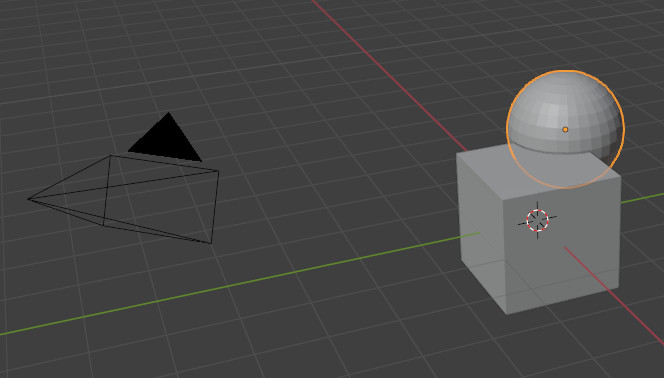
\includegraphics[width=.9\linewidth]{images/user-view.jpg}
\caption{User View}
\end{figure}
\end{column}

\begin{column}{.5\columnwidth}
\begin{figure}[htbp]
\centering
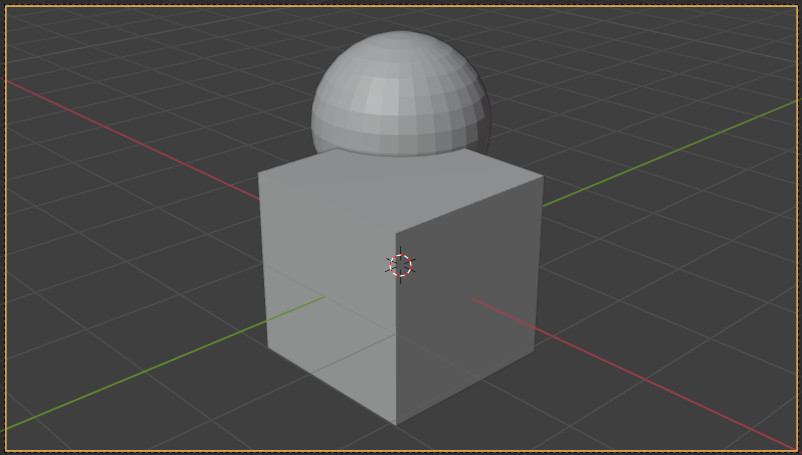
\includegraphics[width=.9\linewidth]{images/camera-view.jpg}
\caption{Camera View}
\end{figure}
\end{column}
\end{columns}
\end{frame}
\begin{frame}[label={sec:org2e62b34}]{interpolation}
\begin{columns}
\begin{column}{.45\columnwidth}
Estimating/ Computing the values in between two states.

\emph{e.g.} \\[0pt]
Points on a line segment are intermediate/ interpolated
states between its two end points.
\end{column}
\end{columns}
\end{frame}

\begin{frame}[label={sec:orgcd4afb0}]{visualisation}
\begin{columns}
\begin{column}{.45\columnwidth}
To create a visible artefact corresponding to a
concept.
\end{column}
\end{columns}
\end{frame}

\section{the graphics pipeline}
\label{sec:org2244030}

\begin{frame}[label={sec:orgea020e3}]{the graphics pipeline}
\begin{columns}
\begin{column}{.3\columnwidth}
\begin{center}
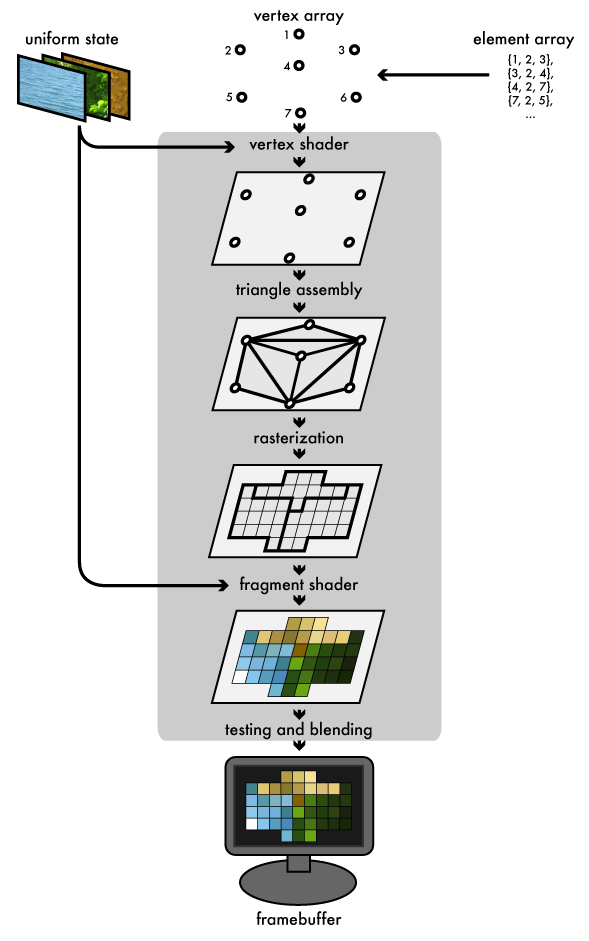
\includegraphics[width=.9\linewidth]{images/gl1-pipeline-01.png}
\end{center}
\tiny \emph{Image Courtesy: \href{https://duriansoftware.com/joe/media/gl1-pipeline-01.png}{Durian Software}}
\end{column}
\begin{column}{.7\columnwidth}
\begin{itemize}[<+>]
\item Data Input
\begin{itemize}[<. | only@.>]
\item Uniform State
\item Vertex Array (per-vertex data)
\item Element Array (list of elements)
\end{itemize}
\item \alert{Vertex Shader}
\begin{description}[<. | only@.>]
\item[{input}] \begin{itemize}
\item Per Vertex Data
\item Uniform State
\end{itemize}
\item[{output}] \begin{itemize}
\item Position
\item For Next Shader
\end{itemize}
\end{description}
\item Triangle Assembly 
\begin{itemize}[<. | only@.>]
\item Uses Element Array
\end{itemize}
\item Rasterisation
\begin{itemize}[<. | only@.>]
\item Which element corresponds to which fragment
\end{itemize}
\item \alert{Fragment Shader}
\begin{description}[<. | only@.>]
\item[{input}] \begin{itemize}
\item From Prev Shader
\item Uniform State
\end{itemize}
\item[{output}] \begin{itemize}
\item Fragment Colour
\end{itemize}
\end{description}
\item Framebuffer
\end{itemize}
\end{column}
\end{columns}
\end{frame}
\subsection{Geometry Definition in OpenGL}
\label{sec:org53f28ee}
\begin{frame}[label={sec:orgb370a4e}]{three types}
\begin{itemize}[<+ | alert@+>]
\item \huge \textsc{point}
\item \huge \textsc{straight line}
\item \huge \textsc{planar polygon}
\normalsize
\begin{itemize}[<. | only@.>]
\item Triangle
\item Quad
\end{itemize}
\end{itemize}
\end{frame}
\begin{frame}[label={sec:org594f87c}]{attributes}
\end{frame}
\begin{frame}[label={sec:orgaa0f0b9}]{elements}
\end{frame}
\subsection{Vertex Shader}
\label{sec:org1ec3a31}
\subsection{Fragment Shader}
\label{sec:orgabb0cdd}
\section{hot rod example}
\label{sec:orgfaa46b5}
\begin{frame}[label={sec:org519b806}]{problem}
\begin{columns}
\begin{column}{.45\columnwidth}
\alert{Given} a straight line with vertex attributes: \emph{a)}
position in 2D coordinates; and \emph{b)} temperature value;

\alert{Draw} the line with a heat gradient using a predefined
heat map for colour.
\end{column}
\end{columns}
\end{frame}

\section*{references}
\label{sec:orge1e3251}
\begin{frame}[allowframebreaks]{references}
\printbibliography
\end{frame}
\end{document}
